% Geometry, font
\documentclass[12pt, letter]{article}
\usepackage[margin=0.8in]{geometry}
\usepackage[T1]{fontenc}
\usepackage{fourier}
\usepackage{titling}
\setlength{\droptitle}{-5em} 
\usepackage[parfill]{parskip}
\usepackage{graphicx}
\usepackage{hyperref}

\usepackage{fancyhdr}
\lhead{ECE 4542: Advanced Engineering Algorithms}
\rhead{Zach Neveu}
\pagestyle{fancy}

% Math stuff
\usepackage{amssymb}
\usepackage{bm}

% Code Highlighting
\usepackage{minted}
\usemintedstyle{solarizedlight}

\title{ Homework 6 }

\begin{document}
\maketitle
\thispagestyle{fancy}

\begin{enumerate}
	\item Dynamic Programming Matrix Multiplication. 	
	\begin{enumerate}
		\item Dynamic Programming Approach. This approach goes through the half-matrix shown in figure \ref{fig:hw6} starting from the diagonal, and working towards the top left corner. The diagonal cells are filled with the matrices to be multiplied. For the row above that, there is only one way to create each cell: simply multiplying the two child cells in order. The third row gets more complicated, because there are two possible ways to parenthesize 3 matrices. The costs for both methods are calculated, and the minimum cost method is chosen. The final row uses the best answers from row 3, and adds the final matrix to calculate a final total. The best cost to multiply the given matrices is 2200 scalar multiplications, and the best parenthesization is (M1(M2*M3))M4.
		\begin{figure}[h]
			\centering
			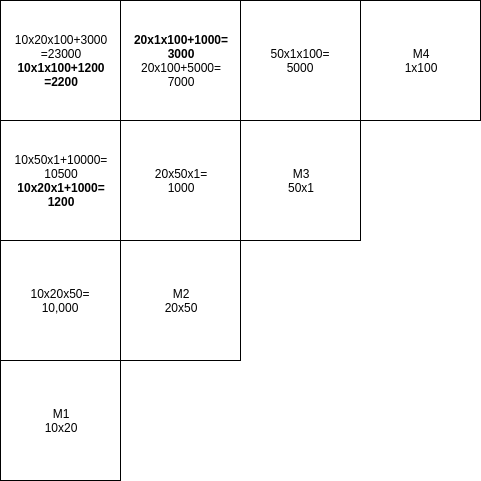
\includegraphics[width=0.6\linewidth]{hw6}
			\caption{Dynamic Programming Half-matrix}
			\label{fig:hw6}
		\end{figure}
		\item Recursive Approach. The code below implements a recursive approach to finding the minimum number of scalar multiplies needed to multiply a chain of matrices. The function will initially be called on the entire chain. This top level call will iterate over all possible places to divide the chain, making recursive calls to solve each of the two subproblems and add the cost of multiplying the results. For example, on the example given, (M1*M2*M3*M4), The initial call would have i=1,j=4 (assuming 1 indexing). The algorithm would first try making recursive calls with i=1,j=1, and i=2,j=4. The first of these calls returns 0, the second call spawns two more calls with i=2,j=2 and i=3,j=4. Once again, the first call returns 0, while the second call is expanded into i=3,j=3 and i=4,j=4 which each return 0. The final term of the cost for this bottom-most call is the cost of M3*M4. For each level of the recursion, all possible k are tried in order to find the best result.
\begin{minted}{Python}
# Recursive Matrix Chain Multiply
def RecurseMatChain(p,i,j):
    if i == j:
        return 0
    else:
        m[i,j] = MAX_INT # set to infinity
        for k in range(i,j-1):
            q = RecurseMatChain(p,i,k)+RecurseMatChain(p,k+1,j)+p[i-1]p[k]p[j]
            if q < m[i,j]:
                m[i,j] = q
    return m[i,j]
\end{minted}

	\end{enumerate}
	\item The advantage of using dynamic programming to solve optimization problems is that it provides a structured way of calculating and saving the results to all of the subproblems needed to solve a larger problem. This ensures that the full solution space is explored, and can be more straightforward to program then hand-coding custom structures for something like branch and bound to remember all past solutions. It can also save a huge amount of time over recursive methods that do not save each subproblem result.
	\item Optimal substructure is a property of certain problems which dynamic programming is designed to make use of. For problems that have optimal substructure, a solution is composed of the solutions to a combination of one or more subproblems. In order for the solution to be optimal, the solution to the subproblems must all be optimal.
	\item \textbf{Memoization:} The process of saving solutions to subproblems in an organized manner in order to avoid duplication of work when solving larger problems.
\end{enumerate}

\end{document}
